\subsubsection{Dynamiske side af analysen}
\begin{figure}[htb!]
  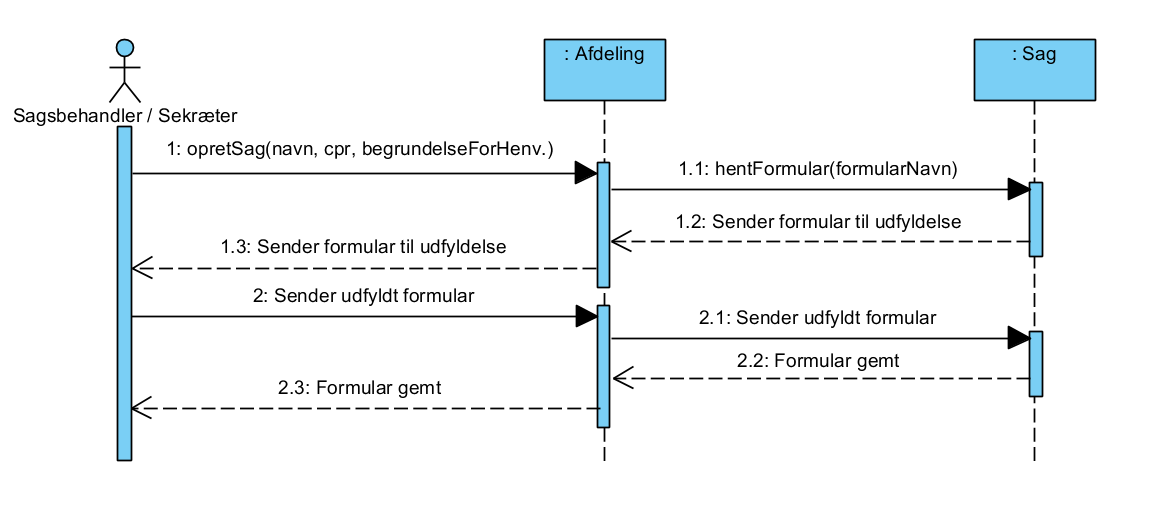
\includegraphics[width=\linewidth]{./PNG/analyse/opretSag.PNG} 
  \caption{Sekvensdiagram for opret sag}
  \label{fig:opretSag}
\end{figure}
\textbf{Opret sag}\\
Beskrivelse:\\
Som man kan se på figur \ref{fig:opretSag} påbegynder operationen opretSag ved at en af aktøren, sagsbehandler eller sekretær anmoder systemet om at oprette en sag til afdeling. Afdelingen håndterer operationen ved at hente en formular ved at sende forespørgsel til Sag objektet. Objektet tilbagesender en pågældende formular tilbage til afdeling objektet. Når afdelingen modtager formularen, videresendes den til den pågældende aktør. Aktøren udfylder formularen med relevante oplysninger, hvorefter den sendes til afdelingen, hvor denne sender det videre til den pågældende sag for opdatering. \\ \\
Evaluering:\\
Det er vigtigt for en sagsbehandler eller sekretær at kunne oprette en sag på en boger. Operationen opretSag er er starten for selve sagsforløbet og dermed essentiel del for systemet. \\
\begin{figure}[htb!]
  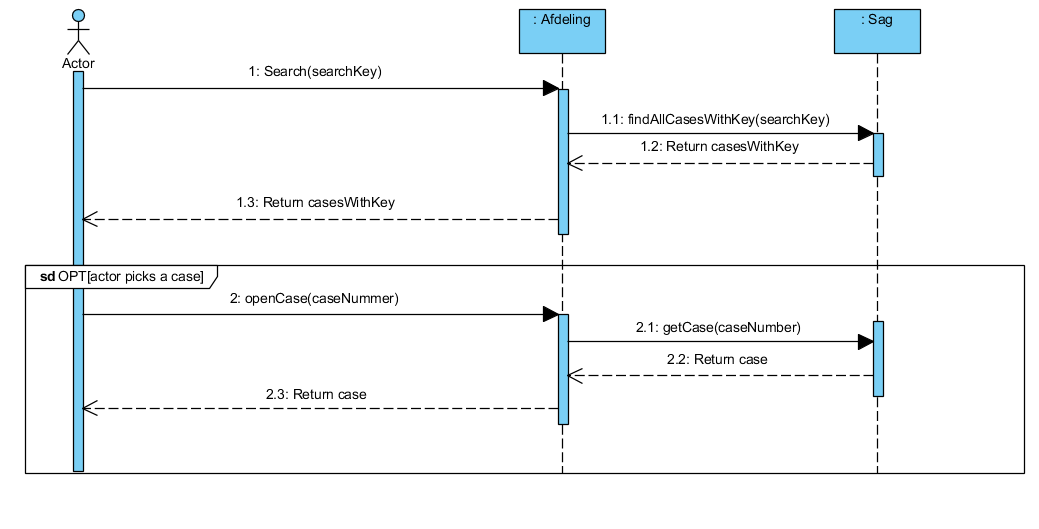
\includegraphics[width=\linewidth]{./PNG/analyse/findSag.PNG} 
  \caption{Sekvensdiagram for find sag}
  \label{fig:findSag}
\end{figure}\\
\textbf{Find sag}\\
Beskrivelse: \\
En aktør, f.eks. sagsbehandler eller sekretær, vælger at søge på en sag, som vist i figur \ref{fig:findSag}. Search metoden modtager en nøgle værdi. Den sender besked ned til afdelingen og herefter spørger en metode efter at finde alle sager med den specifikke nøgleværdi. Sager med den specifikke nøgle sendes tilbage til afdelingen og afdelingen sender resultatet videre til aktøren. Herefter vælger aktøren at åbne den specifikke sag, hvor der kaldes på openCase metoden som sender besked ned til afdelingen. Afdelingen efterspørger herefter om at få den sag med det specifikke sagsnummer, og der returneres et sagsobjekt med det specifikke sagsnummer. Afdelinger returner efterfølgende det fundne sagsobjekt til aktøren. \\ \\
Vurdering:\\
Det er vigtigt for en sagsbehandler eller en sekretær at kunne finde sager vedrørende en borger. Dermed når en borger henvender sig, kan en sekretær søge en sag frem på den pågældende borger.  
